%chapter experiment results
\chapter{Experiment Results \& Justification}
This section is based on lessons learned and any observations made in section \ref{implwhirlpool}.

\section{RabbitMQ Dashboard}

\pagebreak

%\section{Fetcher: Response times for a sample of N requests to 3 different seed servers}

%\pagebreak

\section{Content SeenTest: Near Duplicate Detection}\label{handle_dedupe}
explain LSH
\\
\\
In Summary, when it comes to detecting similarity between two web pages, the pages are converted into
bag of phrases. The challenge lies in storage requirements because the word size for a phrase $p$ adds
a space complexity of O$(np)$, where $n$ is no. of times we have to save the document. Applying a hash
function outputs a integer and is able to improve space complexity of bag of phrases to O$(n)$.
Minhash\cite{dedupe} brings storage requirement to O$(1)$ but time complexity of query documents is
O$(n)$. Simhashing\cite{dedupe} performs better than Minhash by querying on a fix $q$ sorted list of
hashes. Its time complexity is given as O$(q * log(n))$. Efficient Querying and Insertion of simhashes
calls for project implementation of its own.

\pagebreak

\section{Hash based rebalancing}
\begin{figure}[h!]
  \centering
  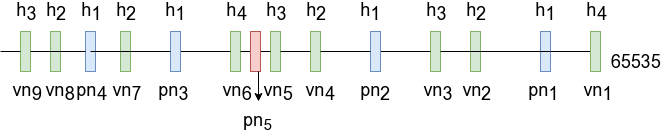
\includegraphics[width=12cm,height=5cm,keepaspectratio]{../media/crawler/addingnode.png}
  \caption{adding new node to existing cluster of nodes}
  \label{fig:addingnode}
\end{figure}

\noindent
Key observation while rebalancing a cluster when adding or removing a node like $pn_5$:
\begin{itemize}
  \item entire vnodes are moved between pnodes
  \item number of vnodes present do not change 
  \item assignment of hash of urls to vnodes do not change
  \item only the assignment of vnodes to pnodes is changed
\end{itemize}

\noindent
The maximum number of pnodes that can be provisioned to manage scalability is equal to total number of
vnodes. At some point if the crawler process changes its property from being just a topical crawler to
also be comprehensive, its compute capacity can get overhauled, thus requiring more horizontal scalability.
Determining how many machines the crawler can outgrow to depends on what needs to be accomplished with the crawler.

\section{MongoDB documents}
\begin{figure}[h!]
  \centering
  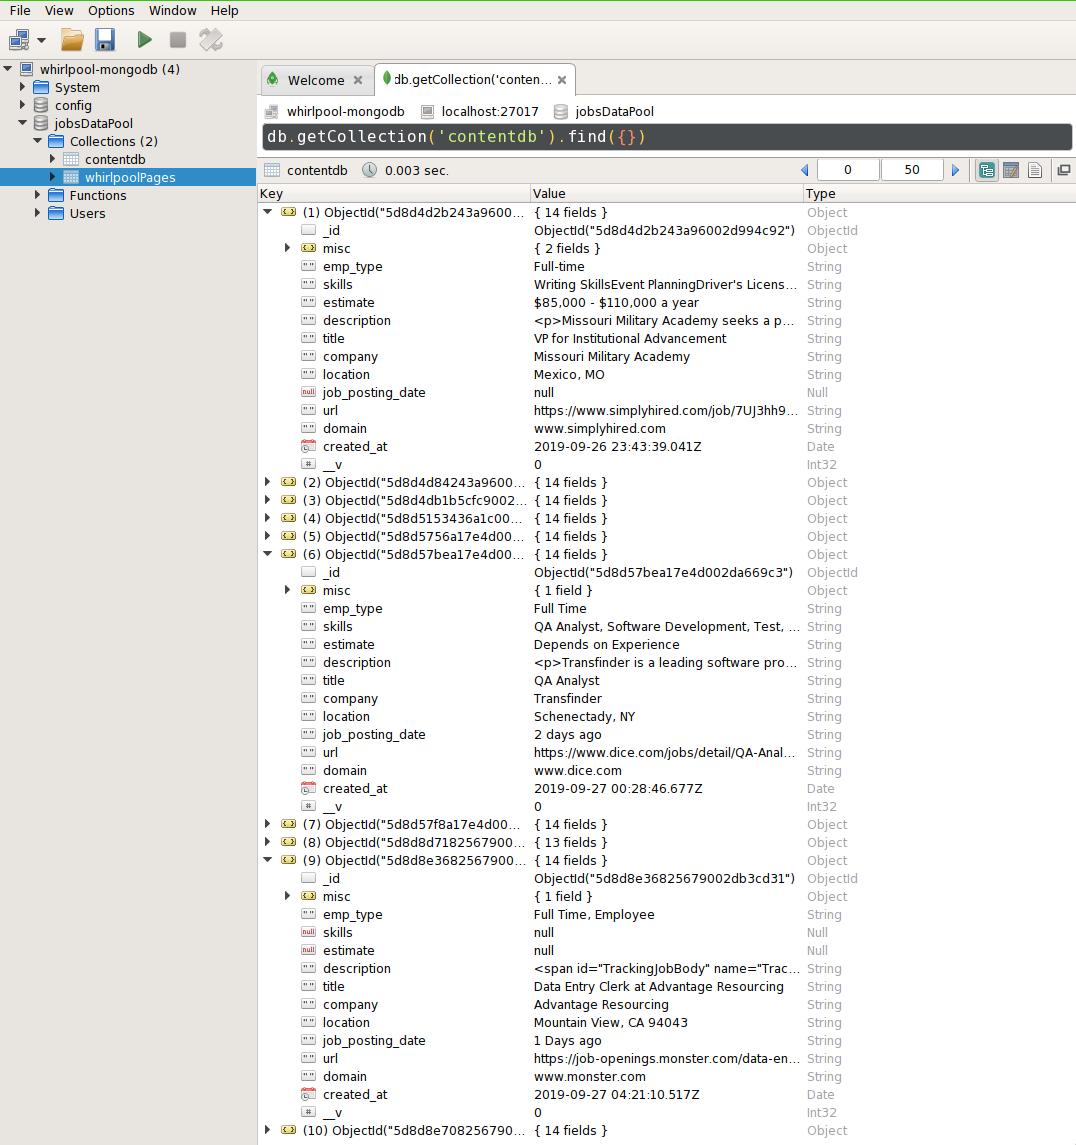
\includegraphics[width=12cm,height=18cm,keepaspectratio]{../media/crawler/collecteddata.png}
  \caption{screenshot of collected data through crawler}
  \label{fig:mongo_data}
\end{figure}
\pagebreak

%\section{Postgres ContentSeen \& DUE Fingerprints}

%\pagebreak

\section{Whirlpool as a Microserivce Application}
To be completed

\pagebreak